


\chapter{Basic multivariate analyses}

\section{The analysis of variance (ANOVA)}
When we are considering three or more groups, we ask whether these groups are different from each other. Another way to think about this is to think about how much of the variance occurs between the groups compared to how much variance occurs within the groups. This ratio is the idea behind ANOVA.

The building blocks of ANOVA is that we can think about each $i^{th}$ case as part of the $j^{th}$ group. We can then conceptualize a way to think about deviance that involves groups.

Here, we can think of the total difference between an observation and the overall mean, $y_{ij}-\bar{y}$, as the difference between that observation and its group's mean, $y_{ij}-\bar{y}_j$, plus the difference between that group's mean and the overall mean, $\bar{y_{j}}-\bar{y}$:
\begin{equation}
y_{ij}-\bar{y} = \left(y_{ij}-\bar{y}_j\right)+\left(\bar{y_{j}}-\bar{y}\right)
\end{equation}
This idea has implications for the sum of squares. We can now think of the total sum of squares ($SST$) as breaking down into the sum of squares within groups ($SSW$) and the sum of squares between groups ($SSB$):
\begin{equation}
SST=SSW+SSB
\end{equation}
or
\begin{equation}
\sum_{j=1}^k\sum_{i=1}^{n_j}\left(y_{ij}-\bar{y}\right)^2=\sum_{j=1}^k\sum_{i=1}^{n_j}\left(y_{ij}-\bar{y}_j\right)^2+\sum_{j=1}^kn_j\left(\bar{y}_j-\bar{y}\right)^2
\end{equation}
There is some new notation here. We now have $k$ groups with the subscript $j$, and each $j^{th}$ group has cases with the subscript $i$.

ANOVA's test statistic relies on the F-distribution to evaluate Type I error. The F-distribution is used to test ratios and is thus defined by two degrees of freedom, one for the numerator and one for the denominator of the ratio, and there are no negative statistics.  As the number of each increases to a large number, the distribution starts to look normal.

As was just mentioned, the test statistic is a ratio. Again, we are concerned with the ratio of the variance that occurs between groups compared to that within groups. Thus, this ratio uses as the numerator the mean square between, which is the sum of squares between divided by the number of groups - 1:
\begin{equation}
MSB=\frac{\sum_{j=1}^kn_j\left(\bar{y}_j-\bar{y}\right)^2}{k-1}
\end{equation}
The denominator of the ratio is the mean square within, which is the sum of squares within divided by the number of cases minus k group means
\begin{equation}
MSW=\frac{\sum_{j=1}^k\sum_{i=1}^{n_j}\left(y_{ij}-\bar{y_{ij}}\right)^2}{N-k}
\end{equation}
The ratio then looks like this
\begin{equation}
F=\frac{MSB}{MSW}
\end{equation}
and we test how much of the $F$-distribution (with $k$ and $N-k$ degrees of freedom) is left after this value for our Type I error rate of our test of the the null hypothesis that all group means are the same. In other words, our null hypothesis is that all the group means are the same:
\begin{equation}
H_0:\mu_1=\mu_2 \ldots =\mu_k.
\end{equation}
Since this distribution has two degrees of freedom parameters, the critical value different for different combinations of $k$ and $N-k$. See Figure~\ref{fig:f} for various distributions.

\subsection{ANOVA Example}

As a cartoony example, let's use political views to predict vocabulary. Or, in less causal language, whether vocabulary varies by political view. These data come from the General Social Survey.

First, we have three political groups, liberal (lib), moderate (mod), and conservative (con). Summary statistics appear in Table~\ref{tab:polstats}.
\begin{table}[htbp]\centering
\caption{Number correct words by political affiliation\label{tab:polstats}
\textbf{} }\begin{tabular} {@{} l r r r @{}} \\
Political affilication &     $N$ & $\bar{y}$ &  $s$ \\
\hline
   lib &   733 &    6.32 &    2.21 \\
   mod &   983 &    5.81 &    1.84 \\
   con &   875 &    6.23 &    1.97 \\
   \hline
  Total &  2591 &    6.10 &    2.01 \\
\hline
\multicolumn{4}{@{}l}{\footnotesize{\emph{Source: General Social Survey: 2008}}}
\end{tabular}
\end{table}

Table~\ref{tab:wordanova} is a typical ANOVA table with the total sum of squares broken down into the sum of squares within and between, with the mean squares also calculated. We can calculate the $F$-test using the mean squares
\[
F=\frac{MSB}{MSW}=\frac{67.216}{3.984}=16.87.
\]
Which, evaluated with $\left(2,2588\right)$ degrees of freedom on the $F$ distribution, has a probability of 0.0000005. This indicates that at least one group is different than the others. To find out which group is different requires some regression analysis.

\begin{table}[htbp]\centering
 \caption{ANOVA of word test by political views
\label{tab:wordanova}}
\begin{tabular}{lrrr}
\hline
Source & Sum of squares & $df$ & Mean Squares \\
\hline
Between groups & 134.432 & 2 & 67.216 \\
Within groups & 10311.878 & 2588 & 3.984 \\
\hline
Total & 10446.31 & 2590 & 4.03 \\
\hline
\multicolumn{4}{l}{Model Statistics} \\
\hline
$N$      &   2591 & \\
$F$      &   16.87  \\
\hline
\end{tabular}
\end{table}

\section{Covariance}
The covariance is a simple idea: instead of squaring the deviance of one variable from its mean, the covariance multiplies the deviances of two variables from their means:
\begin{equation}
  \mbox{cov}\left(y,x\right)=\frac{\sum_{i=1}^N\left(y_i-\bar{y}\right)\left(x_i-\bar{x}\right)}{N-1}
\end{equation}
\begin{table}[htbp]\centering
\caption{Small dataset of random variables\label{tab:xy}
\textbf{} }\begin{tabular} {@{} c c @{}} \\
$y$ & $x$ \\
\hline
 8.20&4.51\\
 9.21&5.36\\
10.22&6.23\\
 8.56&3.84\\
10.66&4.90\\
 9.93&5.00\\
 8.29&4.80\\
 9.18&4.34\\
 9.22&5.78\\
 7.29&4.06\\
\hline
\multicolumn{2}{@{}l}{\footnotesize{\emph{} }}
\end{tabular}
\end{table}
\begin{figure}
   \centering
   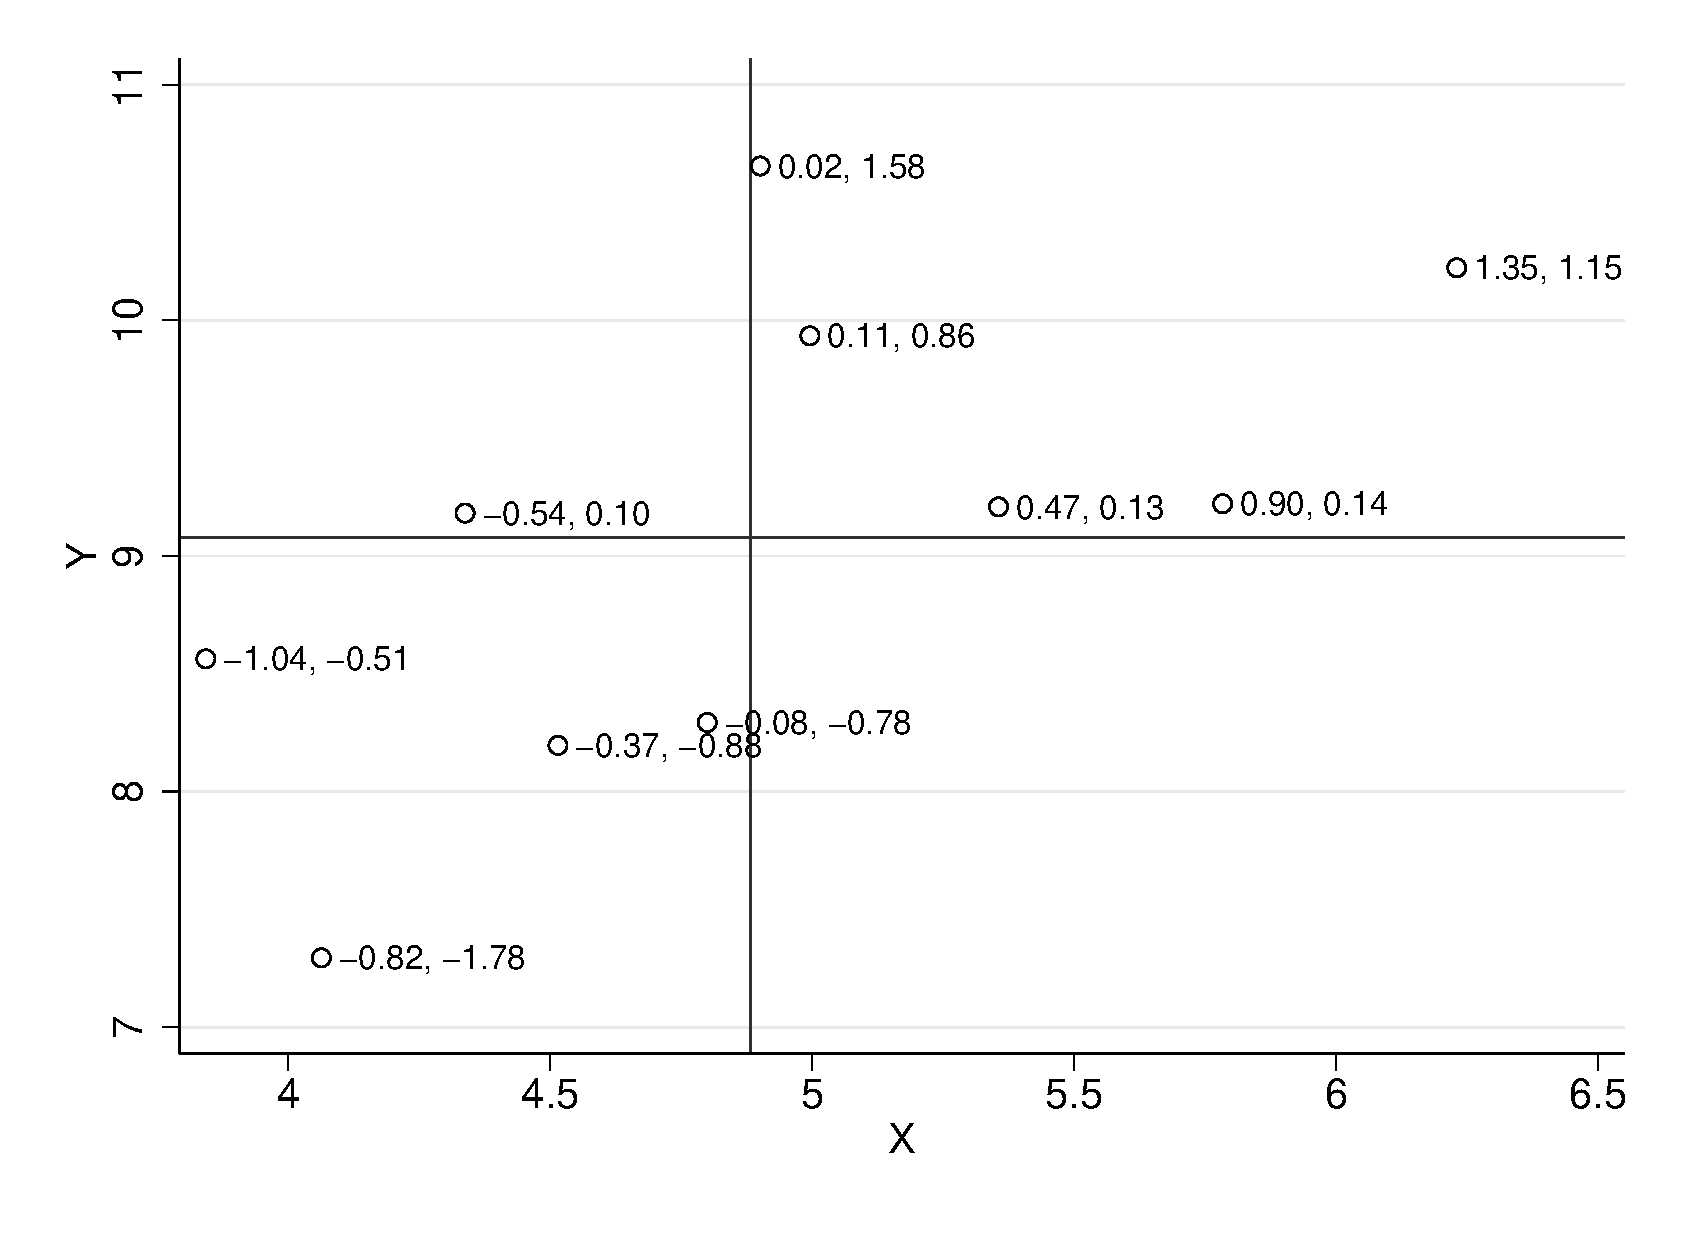
\includegraphics[angle=0,
           width=.75\textwidth]{cov_xy.eps}
   \caption{Plot of variables $y$ and $x$ with solid lines for means, labeled with deviations from the means}
  \label{fig:cov_xy}
\end{figure}
We can visualize this by using a scatterplot. Figure~\ref{fig:cov_xy} is a scatterplot of the data with the means of $x$ and $y$ marked with vertical and horizontal lines and each point marked with the deviations from the mean. The data appear in Table~\ref{tab:xy}.
\begin{figure}
   \centering
   \includegraphics[angle=0,
           width=.75\textwidth]{cov.eps}
   \caption{Covariance quadrants}
  \label{fig:cov}
\end{figure}
Now, consider Figure~\ref{fig:cov}. The means of $x$ and $y$ have been graphed into four quadrants. Each quadrant is defined by the sign of the deviation from the means of $x$ and $y$. Observations whose values of $x$ and $y$ are both larger than the mean of $x$ and $y$ respectively will fall into quadrant one $(+,+)$. Observations whose values have $x$ and $y$ are both lower than the respective means will fall into quadrant three $(-,-)$. The key is that the product of any deviations in either of these quadrants will be positive (a negative times a negative is positive). On the other hand, points that fall into the other quadrants (quadrant two and quadrant four) will have products that are negative (a negative times a positive is negative).

Why do we care about the products of the deviations? Consider the numerator of the covariance formula, $\sum_{i=1}^N\left(y_i-\bar{y}\right)\left(x_i-\bar{x}\right)$. All this is doing is adding up these products. Therefore, more positive products will produce a large positive number, more negative products will produce a large negative number. In addition, larger deviations of either $x$ or $y$ will create larger numbers, and large deviations of both $x$ and $y$ will create a really big number.

If more points fall into the positive quadrants $(+,+; -,-)$ the result is a positive number. If more points fall into the negative quadrants $(-,+;+,-)$, the result is negative. If equal numbers fall into each quadrant, then they will balance out and the number will be close to 0.

Figure~\ref{fig:cov_xy} shows the deviations marked for each point on the scatterplot: what do you think the covariance is?

The denominator of the covariance formula ($N-1$) just turns it into an average, like the variance. Looking at Figure~\ref{fig:cov_xy}, we can tell that the relationship between $x$ and $y$ is positive. The direction of a relationship is generally thought of as what happens to $y$ as $x$ increases. Thus, the covariance in Figure~\ref{fig:cov_xy} is 0.47. This tells me that when $x$ increases, so does $y$. If this number was negative, then as $x$ increases $y$ would decrease.
\section{Correlation}
One of the biggest problems with covariance is that it is really hard to interpret anything meaningful from it. Covariance identifies if the relationship is positive or negative, but it doesn't provide information about the magnitude of the relationship. In addition, the units get all messy. For instance, if the variables were wages and years of education, then the units would be wage-years. What is a wage-year? The solution to this problem is standardization. It would be helpful to standardize this quantity, and one method is to use the sum of squares of the two variables involved. This is basically what the correlation coefficient is about. It is a standardized covariance. The correlation formula is
\begin{equation}
  r_{y,x}=\frac{\sum_{i=1}^N\left(y_i-\bar{y}\right)\left(x_i-\bar{x}\right)}{\sqrt{\sum_{i=1}^N\left(y_i-\bar{y}\right)^2\sum_{i=1}^N\left(x_i-\bar{x}\right)^2}}
\end{equation}
The numerator of this equation is simply the covariance formula while the denominator is the sum of the squares equation. Since the units of the variables are the same for the numerator and denominator, the units cancel out

Correlation coefficients range from -1 to 1. If it is 0, it means that there is no covariance between $x$ and $y$. If it is close to 1, it means that there is a strong positive covariance between $x$ and $y$. If it close to -1, it means that there is a strong negative covariance between $x$ and $y$. All information about the units is lost. It does not matter what $x$ and $y$ are measured by.
\subsection{Testing the correlation coefficient}
\label{sec:introhypo}
What if we wanted to know if our correlation coefficient was {\it statistically} different than 0? In this case, we need to consider the sampling distribution of the correlation coefficient. I go into this in more detail below, but for now remember that we have a random {\it sample}, and if we started our research another day, we would get a different {\it sample}. Thus, the estimated correlation coefficient from our data is one of many possible estimates. We want to know the distribution of these estimates from different hypothetical samples, so we can know how likely our estimate is, assuming a world where a null hypothesis is true. In this case, our null hypothesis is that there is no correlation. For the data in Figure~\ref{fig:cov_xy}, the correlation is 0.61. The question is, is this statistically different than 0?

Since we have a sample, we will rely on the student's $t$ distribution. We can estimate a test statistic for a correlation with
\begin{equation}
t = \frac{|r|\sqrt{N-2}}{\sqrt{1-r^2}}
\end{equation}
which in this case is
\[
t = \frac{0.61\sqrt{10-2}}{\sqrt{1-0.61^2}}
\]
\[
t = 2.18
\]
Now, in our case in Table~\ref{tab:xy}, we have 10 cases, and with 2 means (for two variables) we have 10-2 = 8 degrees of freedom. Figure~\ref{fig:critical} is the sampling distribution of our statistic if we assume that the null hypothesis, or the hypothesis that the correlation is 0, is true. If you look carefully, you will see that the probability of finding a correlation of 0.61 with 10 cases is about 0.06. The math to find that number is a little tedious, so most stats books tell you what test you need to get in order to have a sufficiently low probability to reject the null hypothesis. In our case, that value is about 2.31. Why 2.31? That is a number large enough to claim that if we assume the null hypothesis, the chance of finding that test in our data is less than 0.05. Another way of saying that is that the Type I error rate is less than 5 percent. We sometimes call the Type I error rate $\alpha$ and so we say that $\alpha = 0.05$.

In this case, with a test statistic of 2.18, which is smaller than the critical value of 2.31, we have to accept the null hypothesis. It was close, but not enough.
\begin{figure}
   \centering
   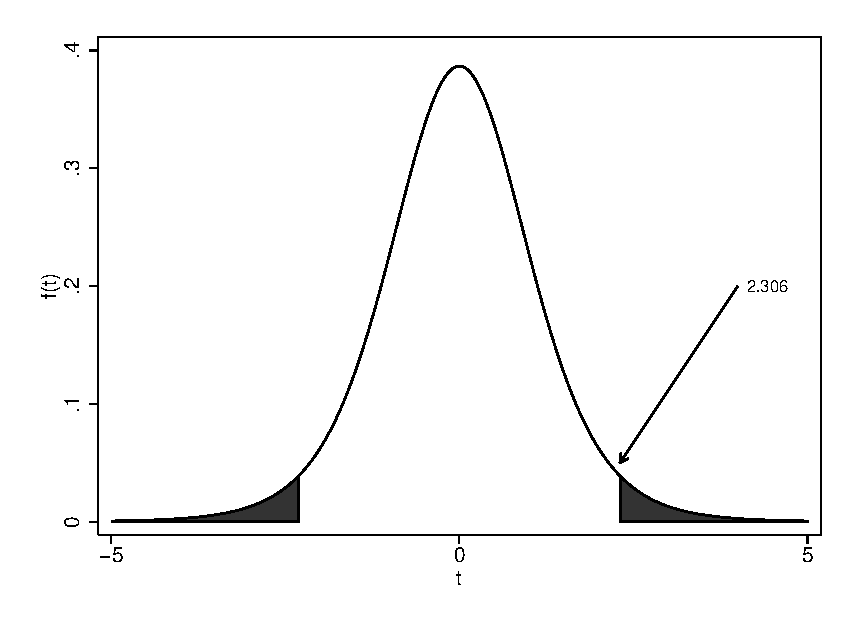
\includegraphics[angle=0,
           width=.75\textwidth]{critical.eps}
   \caption{Plot of $t$ distribution with 8 degrees of freedom and $\alpha$ = 0.05 critical tails marked.}
  \label{fig:critical}
\end{figure}

\section{Chi-square}
In the case of two categorical variables, neither covariance or correlation should be used to determine relationships. Instead, another method based on the idea of deviation is appropriate; the Chi-square $\left(\chi^2\right)$ test. The idea is to state a "null" hypothesis in terms of the researcher's expectation for the results of their analysis. The researcher states what she/he expects, and then offer an alternative hypothesis. If the data deviates in a substantial degree from what the researcher "expects," then the researcher must "fail to reject" the null hypothesis. In common practice, a null hypothesis indicates that there will be no statistically significant relationship between two variables while the alternative hypothesis indicates that there is a statistically significant relationship between the two variables.

The trick to Chi-square tests is that the "expected" value can be anything. You may remember the Chi-square tests from your research methods or statistics class. Frequently, data is presented in table format. In such a table we have (at least) two categorical variables $x$ and $y$. The variable $x$ takes on values such as $x\in\left\{1 \ldots i\right\}$ and variable $y$ takes on values such as $y\in\left\{1 \ldots j\right\}$. Each cell in the table has a number of observations associated with it, $n_{ij}$, for a total of $N=\sum_i\sum_jn_{ij}$ observations. In the case of a two variable table, $x$ makes up the rows and $y$ makes up the columns. We also have totals for each row, $n_{i+}$, and for each column, $n_{+j}$. Chi-square tests then make a comparison between the observed frequency, $n_{ij}$ and what the researcher "expects" each cell frequency to be, $m_{ij}$. This test is
\begin{equation}
\chi^2=\sum_i{\sum_j{\frac{\left(n_{ij}-m_{ij}\right)^2}{m_{ij}}}}.
\end{equation}
A big value for this number tells us that there is a difference between our data and our expectation. Depending on what we are doing, this expectation is different. If we are testing to see if two variables are independent, when we test against a random expectation, or we expect the cells to simply be a function of the margins. So, in this case, $m_{ij}$ is
\begin{equation}
m_{ij}=\frac{n_{i+}n_{+j}}{N}
\end{equation}
So, what's a big value? In this case, it depends on how many cells are in the table. Any statistical test is compared to a function, generally based on some degrees of freedom. For example, a Chi-square test is compared against a Chi-square distribution with $\left(rows-1\right)\left(columns-1\right)$ degrees of freedom. If the value of the test is far enough along that distribution to be considered unlikely if the expectation is true, then we reject the expectation. For example, a $2\times2$ table has a single degree of freedom and a critical value of 3.84 for a Type I error rate of 0.05. Figure~\ref{fig:chi} display some $\chi^2$ distributions.
